\documentclass[18pt]{extarticle}

\usepackage{amsmath}
\usepackage{titlesec}
\usepackage{ifthen}
\usepackage{fancyhdr}
\usepackage{amsmath}
\usepackage{graphicx}

\usepackage{listings}
\usepackage{color}

\usepackage[utf8]{inputenc}
\usepackage{amsmath}
\usepackage{amsfonts}
\usepackage{amssymb}
\usepackage{graphicx}
\usepackage{booktabs}
\usepackage{algorithm}
\usepackage{algpseudocode}
\usepackage{subcaption}
\usepackage[english]{babel}
\usepackage[export]{adjustbox}
\usepackage{enumerate}
\usepackage[left=3.5cm,right=2.5cm,top=2.5cm,bottom=2.5cm]{geometry}
\usepackage{lineno}
\usepackage{cite}
\usepackage{acronym}
\renewcommand{\baselinestretch}{1.5}

\definecolor{dkgreen}{rgb}{0,0.6,0}
\definecolor{gray}{rgb}{0.5,0.5,0.5}
\definecolor{mauve}{rgb}{0.58,0,0.82}

\lstset{frame=tb,
	language=Python,
	aboveskip=3mm,
	belowskip=3mm,
	showstringspaces=false,
	columns=flexible,
	basicstyle={\small\ttfamily},
	numbers=none,
	numberstyle=\tiny\color{gray},
	keywordstyle=\color{blue},
	commentstyle=\color{dkgreen},
	stringstyle=\color{mauve},
	breaklines=true,
	breakatwhitespace=true,
	tabsize=3
}



%opening
\begin{document}
\begin{center}
	\begin{LARGE}			\bf{Programming Assignment \#2\\}
	\end{LARGE}
	\vspace*{30pt}
	
	
	\vspace{20pt}
	\textbf{Medical Equipment II\\}
	\vspace{40pt}
	
	\textbf{
		Ahmed Khaled Mohamed Salah \hspace*{10mm} S.1  B.N.4\\
		Eslam Khaled Korany \hspace*{26mm} S.1  B.N.13\\
		Bassam Moustafa Mahmoud \hspace*{15mm} S.1  B.N.22\\
		Tarek Allam Ibrahim \hspace*{26mm} S.2  B.N.2\\
	}
		\vspace{30pt}

	\vspace{30pt}
	\textit{Under the kind guidance of}\\
	\textbf{Dr. Inas Ahmed Yassine
	}\\
	
	
	\vspace{20pt}
	
	
	

\end{center}
\pagebreak



\section{Non-Uniformity Effect on the Trajectory}
\textbf{Note: Please make sure of installing pyqt (command in dependencies.txt) to be able to run the program.}
\\The non-uniformity of B causes changes in the Larmor frequency $\omega$ of the molecules as
\begin{equation*}
\omega = \gamma * B
\end{equation*}
where $\gamma$ is the gyromagnetic ratio of the nuclei.
Adding the non-uniformity effect would make our equation
\begin{equation*}
\omega ^{'} = \omega + \delta \omega = \gamma * (B + \delta B)
\end{equation*}

For our example we have $B = 1.5 T$ and $\delta B = \pm 1$. So, $B_+ = 2.5 T$ and $B_- = 0.5 T$
A change to the Larmor frequency $\delta \omega$ occurs
\begin{equation*}
\delta \omega = \omega ^{'} - \omega = \gamma * (B + \delta B) - \gamma * B = \gamma * \delta B
\end{equation*}
\begin{equation*}
\delta \omega = \pm 1 * \gamma
\end{equation*}
For protons, $\gamma = 42 MHz.T^{-1}$
\newline
\begin{lstlisting}
B = 1.5
BPositive = 2.5
BNegative = 0.5
gyroRatio = 42
w = gyroRatio * B
wPositive = gyroRatio * BPositive
wNegative = gyroRatio * BNegative
T1 = 490/1000
T2 = 43/1000
t = np.arange(start=0, stop=10, step=0.001)

omega = 2*np.pi*w*t
omegaPositive = 2*np.pi*wPositive*t + np.pi/8
omegaNegative = 2*np.pi*wNegative*t - np.pi/8
\end{lstlisting}


For precising of the protons in the X-Y plane
\begin{equation*}
M_x(t) / M_o = e^{-\frac{t}{T_2}} \sin (\omega t)
\end{equation*}

\begin{equation*}
M_y(t) / M_o = e^{-\frac{t}{T_2}} \cos (\omega t)
\end{equation*}

When there is a non-uniformity in $B$, hence, in $\omega$,
\begin{equation*}
M_x^{'}(t) / M_o = e^{-\frac{t}{T_2}} \sin (\omega^{'} t)
\end{equation*}
\begin{equation*}
M_y^{'}(t) / M_o = e^{-\frac{t}{T_2}} \cos (\omega^{'} t)
\end{equation*}
\begin{lstlisting}
Mx = np.exp(-1*t/T2)*np.sin(omega)
MxPositive = np.exp(-1*t/T2)*np.sin(omegaPositive)
MxNegative = np.exp(-1*t/T2)*np.sin(omegaNegative)


My = np.exp(-1*t/T2)*np.cos(omega)
MyPositive = np.exp(-1*t/T2)*np.cos(omegaPositive)
MyNegative = np.exp(-1*t/T2)*np.cos(omegaNegative)
\end{lstlisting}
Plotting the results of $M_x$, $M_y$ and $M_{xy}$ with the non-uniformity effects for each, we get these results,
\begin{center}
	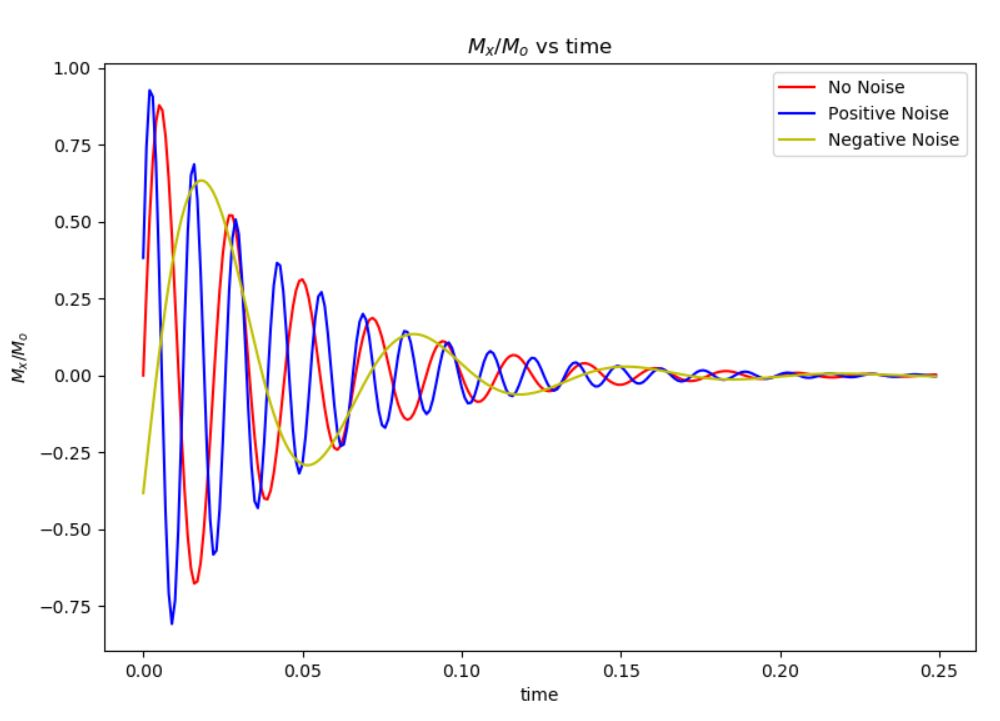
\includegraphics[width=15cm, height=7cm]{mx}
\end{center}
\begin{center}
	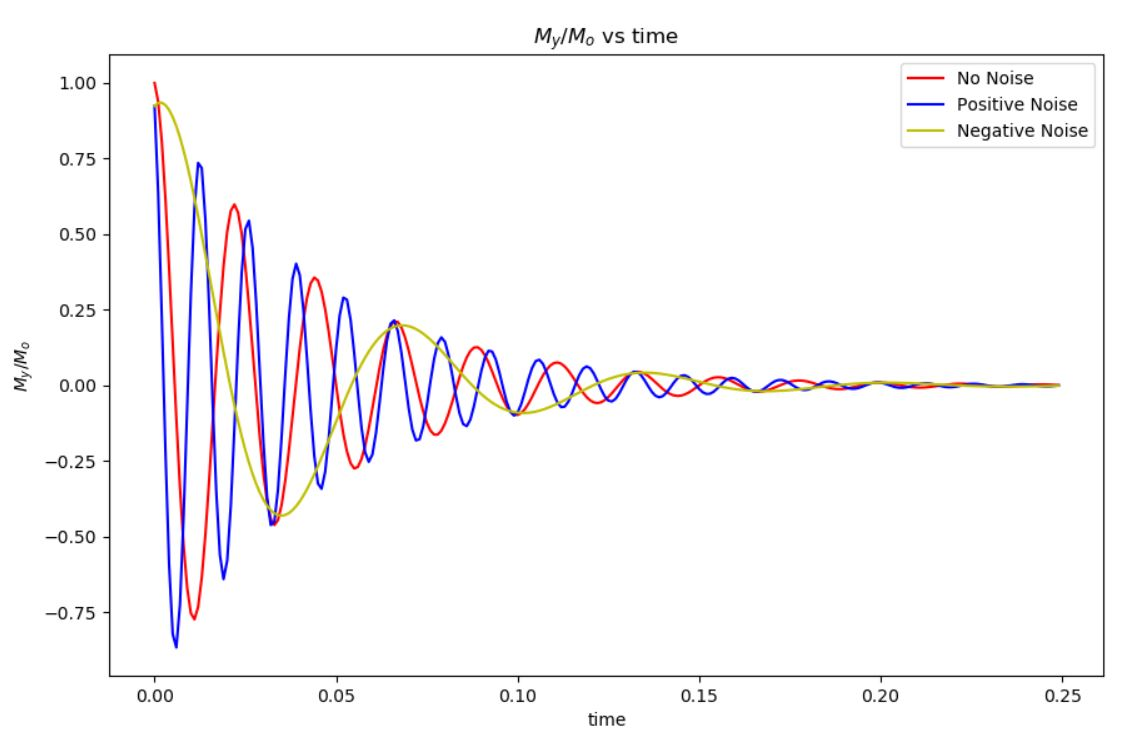
\includegraphics[width=15cm, height=7cm]{my}
\end{center}
\begin{center}
	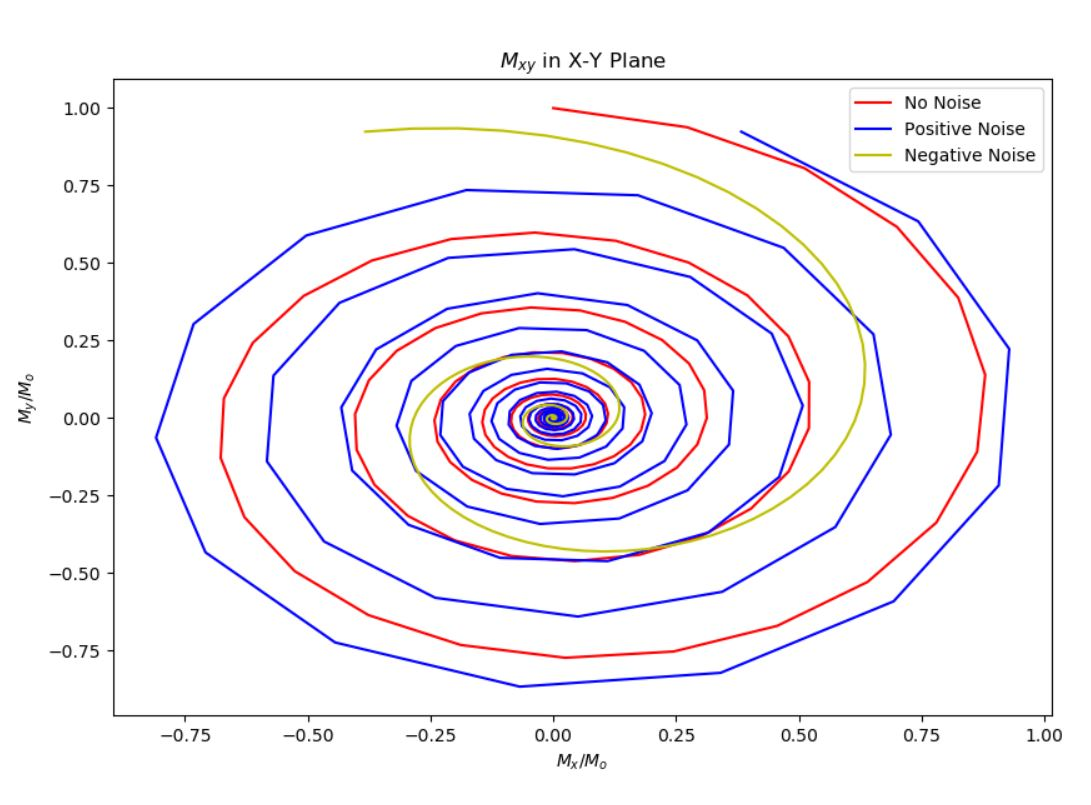
\includegraphics[width=15cm, height=10cm]{mxy}
\end{center}

\section{K-space}
\hspace*{6mm}\large K-space is an array of numbers representing spatial frequencies in the MR image.
Each number's value represents the relative contribution of its unique spatial frequency to the final image.
The k-space and MR image may be converted to one another using the \textbf{Fourier Transform}. The cells of k-space are commonly displayed on rectangular grid with principal axes $k_x$ and $k_y$. The $k_x$ and $k_y$ axes of k-space correspond to the horizontal (x-) and vertical (y-) axes of the image.
\par
\large \textbf{Note}: The individual points ($k_x$,$k_y$) in k-space do not correspond one-to-one with individual pixels (x,y) in the image. Each k-space point contains spatial frequency and phase information about \textbf{every} pixel in the final image.




\end{document}
